%%%%%%%%%%%%%%%%%%%%%%%%%%%%%%%%%%%%%%%%%
% Short Sectioned Assignment LaTeX Template Version 1.0 (5/5/12)
% This template has been downloaded from: http://www.LaTeXTemplates.com
% Original author:  Frits Wenneker (http://www.howtotex.com)
% License: CC BY-NC-SA 3.0 (http://creativecommons.org/licenses/by-nc-sa/3.0/)
%%%%%%%%%%%%%%%%%%%%%%%%%%%%%%%%%%%%%%%%%

%----------------------------------------------------------------------------------------
%	PACKAGES AND OTHER DOCUMENT CONFIGURATIONS
%----------------------------------------------------------------------------------------

\documentclass[paper=a4, fontsize=11pt]{scrartcl} % A4 paper and 11pt font size

% ---- Entrada y salida de texto -----

\usepackage[T1]{fontenc} % Use 8-bit encoding that has 256 glyphs
\usepackage[utf8]{inputenc}
%\usepackage{fourier} % Use the Adobe Utopia font for the document - comment this line to return to the LaTeX default

% ---- Idioma --------

\usepackage[spanish, es-tabla]{babel} % Selecciona el español para palabras introducidas automáticamente, p.ej. "septiembre" en la fecha y especifica que se use la palabra Tabla en vez de Cuadro

% ---- Otros paquetes ----

\usepackage{amsmath,amsfonts,amsthm} % Math packages
%\usepackage{graphics,graphicx, floatrow} %para incluir imágenes y notas en las imágenes
\usepackage{graphics,graphicx, float, url} %para incluir imágenes y colocarlas

% Para hacer tablas comlejas
%\usepackage{multirow}
%\usepackage{threeparttable}
\usepackage{float}


%\usepackage{sectsty} % Allows customizing section commands
%\allsectionsfont{\centering \normalfont\scshape} % Make all sections centered, the default font and small caps

\usepackage{fancyhdr} % Custom headers and footers
\pagestyle{fancyplain} % Makes all pages in the document conform to the custom headers and footers
\fancyhead{} % No page header - if you want one, create it in the same way as the footers below
\fancyfoot[L]{} % Empty left footer
\fancyfoot[C]{} % Empty center footer
\fancyfoot[R]{\thepage} % Page numbering for right footer
\renewcommand{\headrulewidth}{0pt} % Remove header underlines
\renewcommand{\footrulewidth}{0pt} % Remove footer underlines
\setlength{\headheight}{13.6pt} % Customize the height of the header

\numberwithin{equation}{section} % Number equations within sections (i.e. 1.1, 1.2, 2.1, 2.2 instead of 1, 2, 3, 4)
\numberwithin{figure}{section} % Number figures within sections (i.e. 1.1, 1.2, 2.1, 2.2 instead of 1, 2, 3, 4)
\numberwithin{table}{section} % Number tables within sections (i.e. 1.1, 1.2, 2.1, 2.2 instead of 1, 2, 3, 4)

\setlength\parindent{0pt} % Removes all indentation from paragraphs - comment this line for an assignment with lots of text

\newcommand{\horrule}[1]{\rule{\linewidth}{#1}} % Create horizontal rule command with 1 argument of height


\title{	
	\normalfont \normalsize 
	\textsc{{\bf Ingeniería de Servidores (2015-2016)} \\ Grado en Ingeniería Informática y Matemáticas \\ Universidad de Granada} \\ [25pt] % Your university, school and/or department name(s)
	\horrule{0.5pt} \\[0.4cm] % Thin top horizontal rule
	\huge Memoria Práctica 3 \\ % The assignment title
	\horrule{2pt} \\[0.5cm] % Thick bottom horizontal rule
}

\author{Iván Sevillano García} % Nombre y apellidos

\date{\normalsize\today} % Incluye la fecha actual

\begin{document}

\maketitle % Muestra el Título

\newpage %inserta un salto de página

\tableofcontents % para generar el índice de contenidos

\newpage

\section{Conociendo el subsistema de archivos.}

\subsection{Monitorización de Sistemas Linux}

\begin{itemize}
	\item \textbf{¿Qué archivo le permite ver qué programas se han instalado con el gestor de paquetes?}\\
	En el directorio $/var/log/apt/$,donde se encuentran los archivos history.log y term.log. Además, encontramos también archivos con los mismos nombres con las extensiones que abajo se especifican(donde podemos encontrar cualquier número como extensión).
	
	\item \textbf{¿Qué significan las terminaciones .1.gz o .2.gz de los archivos en ese directorio?}\\
	Cada vez que llenamos lo suficiente nuestro archivo history.log, el sistema la comprime y crea un nuevo history.log para almacenar la información sobre nuevos paquetes que instalemos. Las extensiones con distinto número no son más que formas de numerar los distintos paquetes por orden. El orden que siguen va desde el más reciente (extensión .1.gz) hasta el más antiguo.
	
\end{itemize}

\subsection{Programación de tareas con cron}
\begin{itemize}
	\item \textbf{¿Qué archivo ha de modificar para programar una tarea? Escriba la línea necesaria para ejecutar una vez al día una copia del directorio ~/$codigo$ a ~/$seguridad$/$fecha$ donde $fecha$ es la fecha actual (puede usar el comando date)}\\
	Según \cite{crontab}, debemos modificar los archivos en $/var/spool/cron/crontabs/$, sin embargo no están hechos para ser modificados directamente. Se nos ofrece, para modificar el archivo de programación de tareas, el comando $crontab$, que con la opción $-e$, nos deja modificar desde la terminal con el editor de texto que prefiramos.\\
	
	La linea que debemos añadir será la siguiente:\\
	
	00 0 * * *  /$home$/$ivan$/$script.sh$\\
	
	en donde script.sh tiene permisos de ejecución y es el siguiente:\\
	
	\#!/bin/bash\\
	cp -r ~/codigo ~/seguridad/`date +\%y\%m\%d\%H\%M\%S`\\
	
	
	Los primeros cinco $items$ de la sentencia indican cuando queremos que se realice la tarea que se muestra a continuación, por este orden: minuto hora diaDelMes Mes DiaDeLaSemana. No hay que especificar todos los campos, ya que el poner un asterisco($*$) nos dice que no tenga en cuenta este campo. Por ello, en nuestra sentencia, queremos que se ejecute el comando siempre que sean las doce de la noche, sea el día que sea, el mes que sea y el día de la semana que sea. El parámetro `date` nos sirve para cambiar el nombre del archivo a la fecha actual y así tener archivos con distinto nombre.
\end{itemize}

\subsection{Analizando que ocurre en el Kernel con Dmesg}

\begin{itemize}
	\item \textbf{Pruebe a ejecutar el comando, conectar un dispositivo USB y vuelva a
		ejecutar el comando. Copie y pegue la salida del comando (considere usar dmesg |
		tail). Comente qué observa en la información mostrada.}\\
	
	\begin{figure}[H]
		\centering
		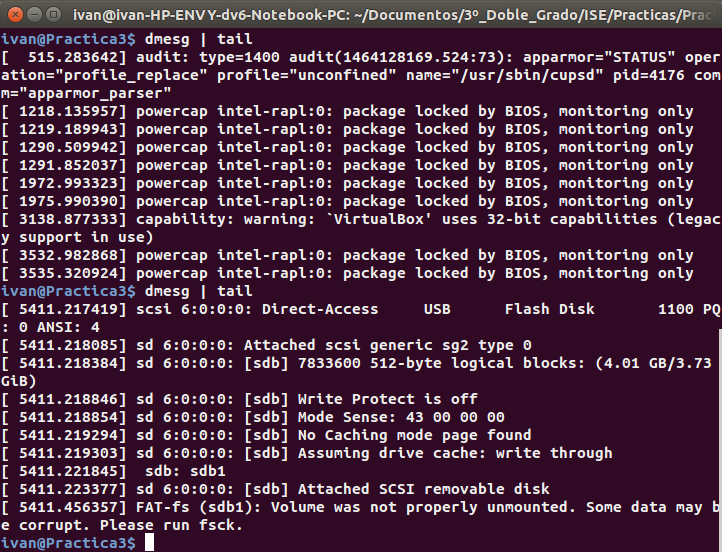
\includegraphics[width=0.7\linewidth]{dmesgPenDrive}
		\caption[dmesg]{Mensaje mostrado por dmesg antes y después de conectar un pen-drive}
		\label{fig:dmesgPenDrive}
	\end{figure}
	
	Antes de conectar el pen-drive, no teníamos ninguna referencia del mismo. Tras conectarlo, el primer mensaje que se nos muestra es la presencia del mismo. También se nos muestran detalles como la capacidad del USB y el uso de la misma(4.01 GB/3.73 GiB) o que se puede escribir en el mismo. En la última línea nos dice que el disco no fue debidamente desmontado.

	
\end{itemize}
\newpage
\section{Monitorización con Windows.}
\begin{itemize}
		\item \textbf{Ejecute el monitor de “System Performance” y muestre el resultado. Incluya capturas de pantalla comentando la información que aparece.}\\
		Al ejecutar el monitor de rendimiento de windows, nos aparece la siguiente interfaz general:\\
		
		\begin{figure}[H]
		\centering
		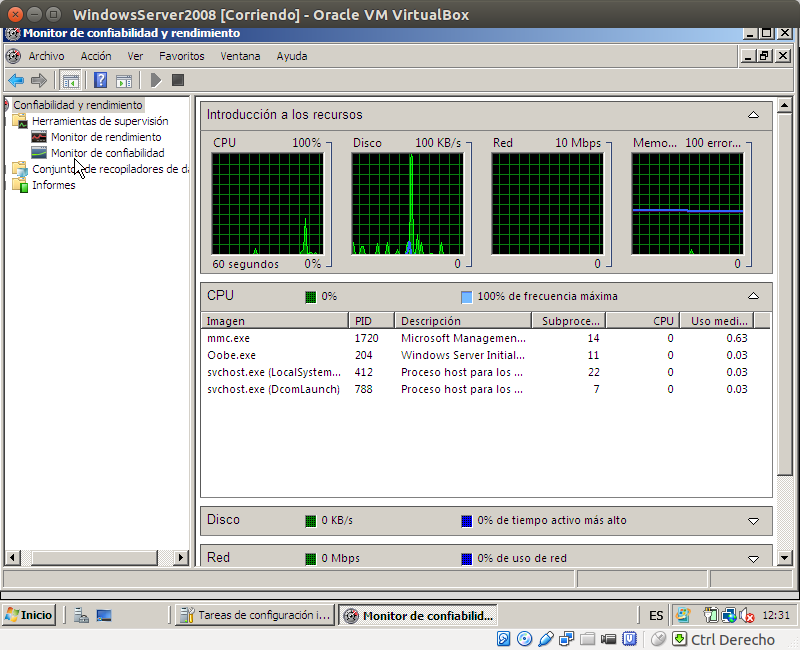
\includegraphics[width=0.6\linewidth]{WindowsCPU}
		\caption[WindowsMonitor]{Monitor de rendimiento en Windows.}
		\label{fig:Profiling_windows}
		\end{figure}
		
		en donde vemos de forma general el rendimiento que está teniendo el sistema. Si queremos enfocarnos en algún campo en concreto haremos click en la gráfica la cuál esté monitorizando el componente que nos interese. Por ejemplo, para obtener información del porcentaje de CPU usado:\\
		
		\begin{figure}[H]
		\centering
		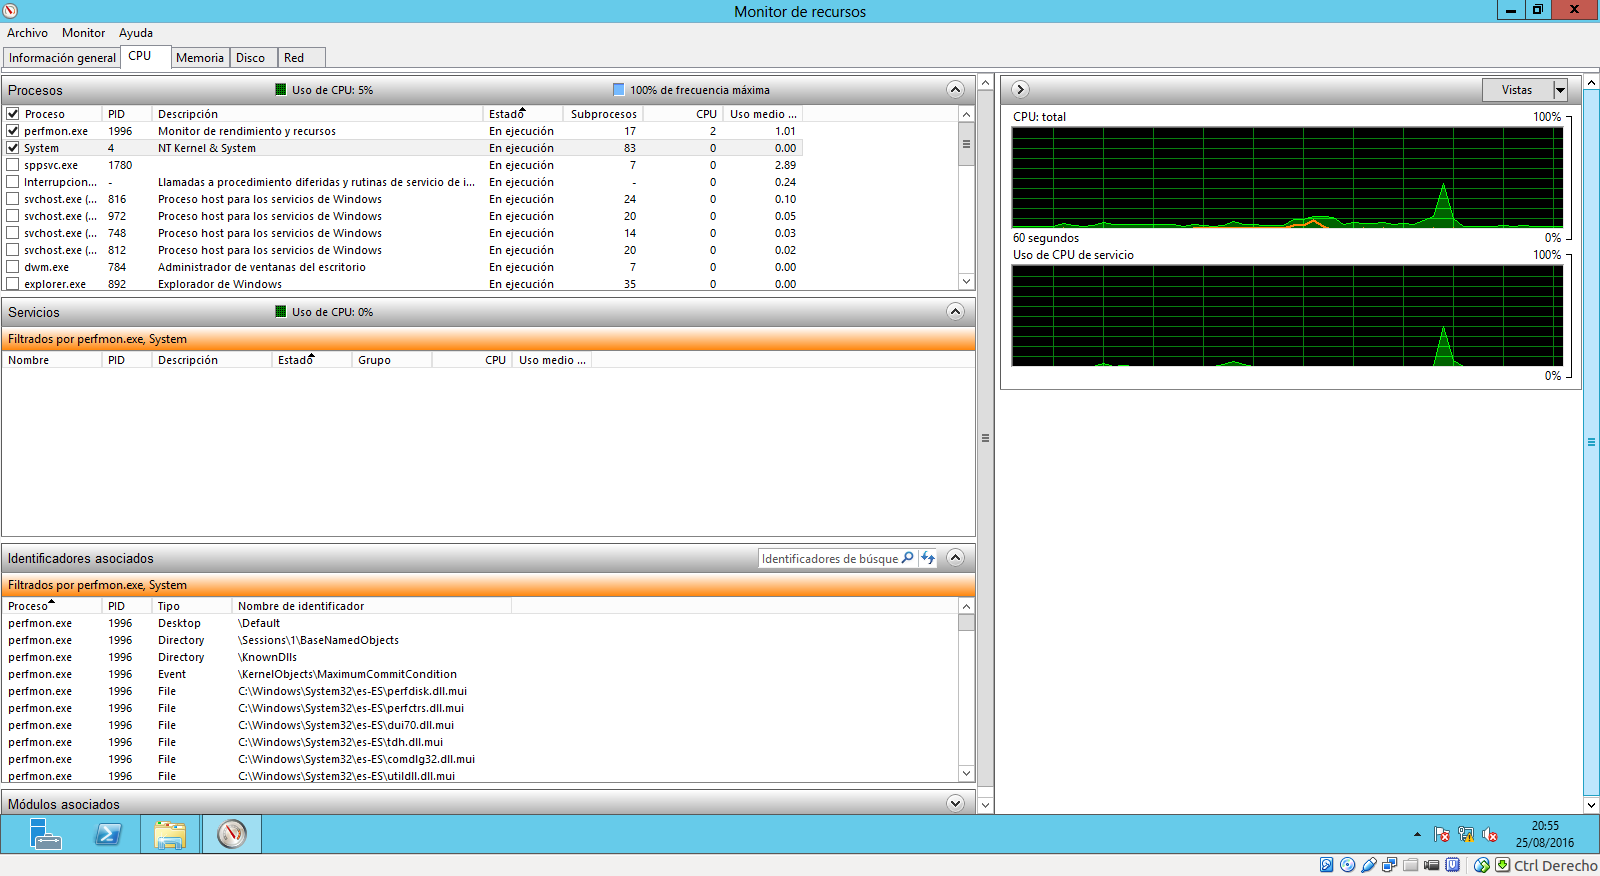
\includegraphics[width=0.6\linewidth]{WindowsCPU2}
		\caption[WindowsCPU]{Uso de la CPU en windows.}
		\label{fig:WindowsCPU}
		\end{figure}
		
		en donde se ve en las gráficas que el uso de la CPU está por debajo del 50\% desde hace 60 segundos.\\
		
		Para obtener datos de la memoria usada por windows:\\
		
		\begin{figure}[H]
			\centering
			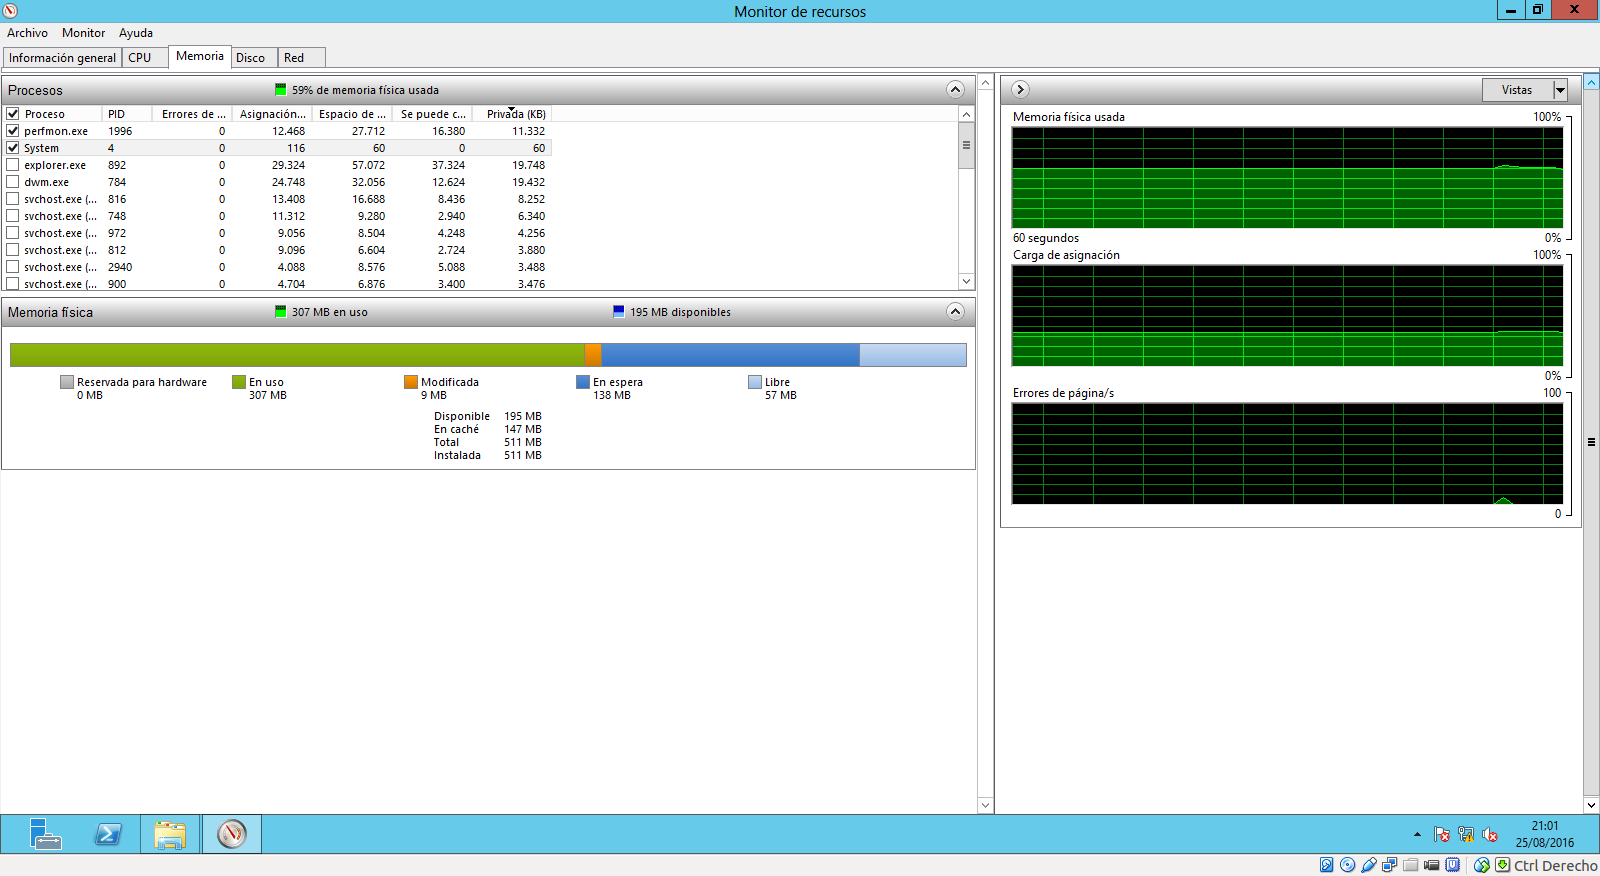
\includegraphics[width=0.7\linewidth]{WindowsMemoria}
			\caption[Windows memoria]{Uso de la memoria total de Windows.}
			\label{fig:WindowsMemoria}
		\end{figure}
		
		en concreto, se ve que en nuestra máquina virtual se está usando mas de la mitad de la memoria que le hemos dado, que hay 195Mb de memoria disponible y 147 en caché.

		
		
		\item \textbf{Cree un recopilador de datos definido por el usuario (modo avanzado) que incluya tanto el contador de rendimiento como los datos de seguimiento: todos los referentes al procesador, al proceso y al servicio web, con un intervalo de muestra de 15 segundos y que almacene el resultado en el directorio $/Escritorio/logs$. Incluya las capturas de pantalla de cada paso.}\\
		
		Para empezar a crear un recopilador de datos clicamos dentro del rendimiento del sistema en recopilador de datos y creamos un nuevo recopilador de datos creado por el usuario:\\
		
		\begin{figure}[H]
		\centering
		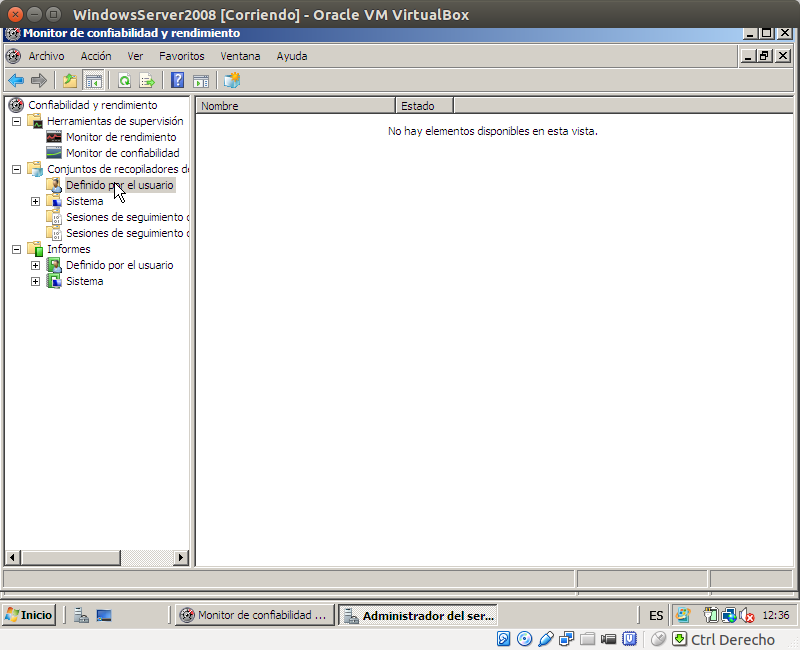
\includegraphics[width=0.6\linewidth]{recopiladorDatos}
		\caption[recopilador Datos]{Donde encontrar la creación del recopilador de datos.}
		\label{fig:recopiladorDatos}
		\end{figure}

		
		Tras esto, se nos pregunta de qué campos tiene que recopilar datos el sistema, en nuestro caso, los datos referentes al contador de rendimiento como los datos de seguimiento.\\
		\begin{figure}[H]
			\centering
			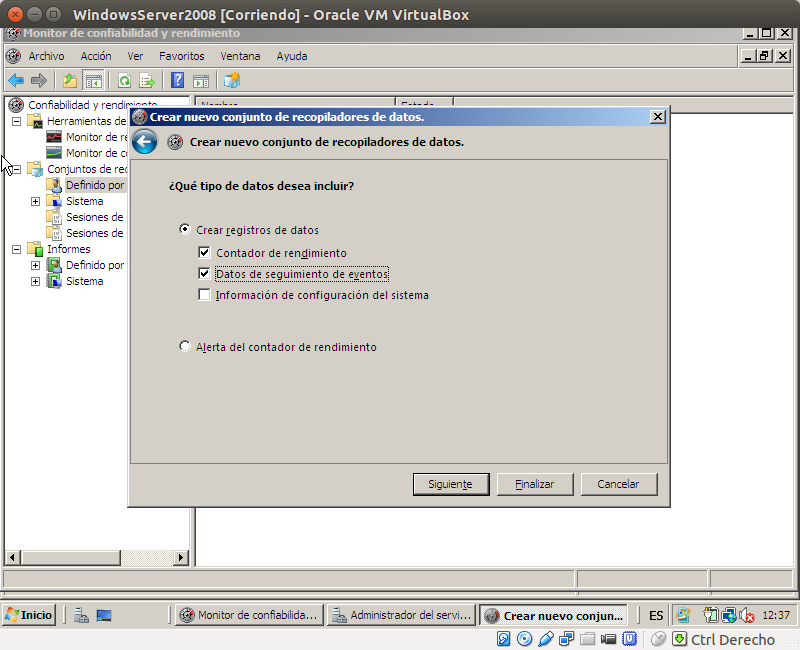
\includegraphics[width=0.6\linewidth]{InicioRecopiladorDatos}
			\caption[RecopiladorDatos]{Inicio de creación y ubicación del recopilador de datos.}
			\label{fig:InicioRecopiladorDatos}
		\end{figure}
		
		Se nos pregunta ahora sobre que componentes vamos a monitorizar. Nosotros escogemos los referentes a los procesos, procesamiento y servicio web:\\
		\begin{figure}[H]
		\centering
		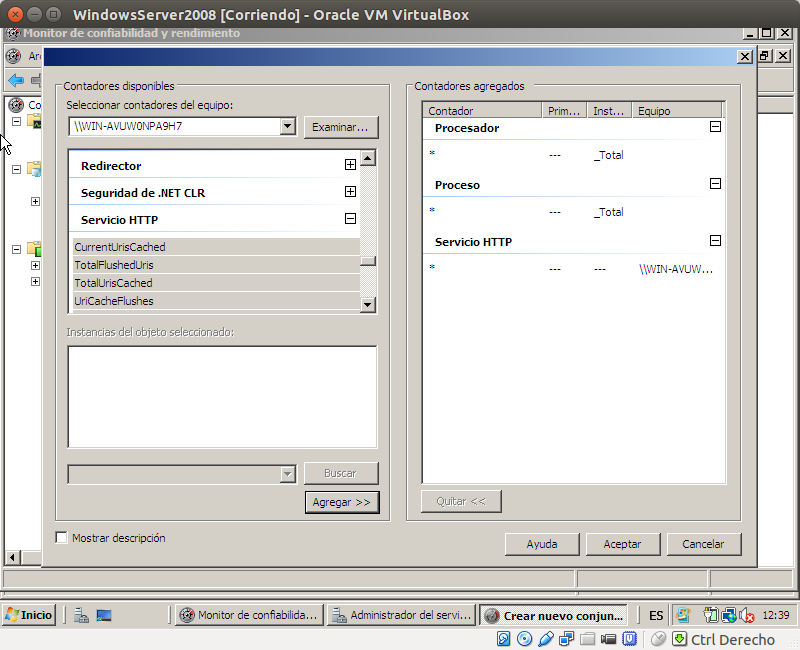
\includegraphics[width=0.6\linewidth]{MonitorizarWindowsServicios}
		\caption[ServiciosWindows]{Escogiendo los componentes a monitorizar.}
		\label{fig:MonitorizarWindowsServicios}
		\end{figure}
		
		A la hora de darle a aceptar, la opción por defecto de tiempo para monitorizar el sistema de 15 segundos:\\
		\begin{figure}[H]
		\centering
		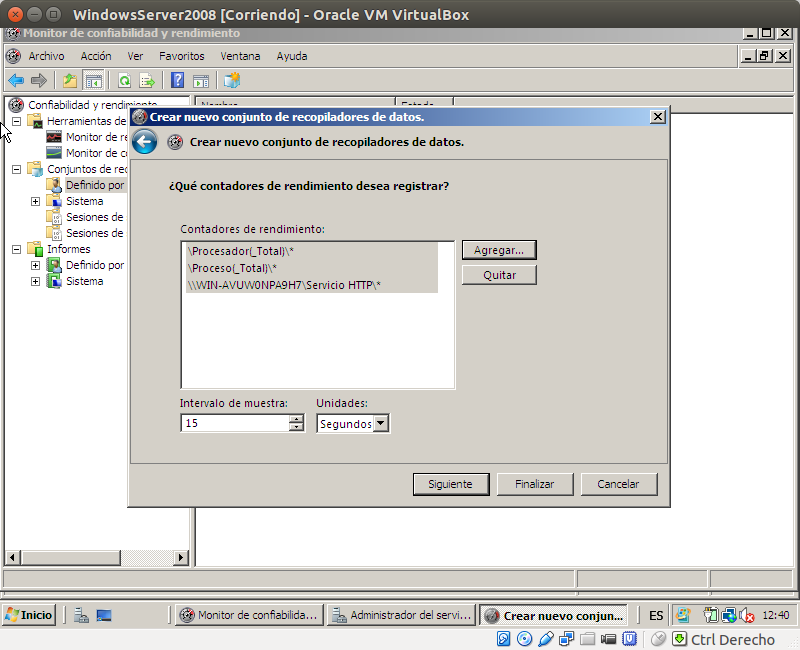
\includegraphics[width=0.6\linewidth]{Intervalo15seg}
		\caption[intervalos]{Intervalos de tiempo para obtener mediciones.}
		\label{fig:Intervalo15seg}
		\end{figure}
		Por último, se nos pregunta donde queremos guardar los datos:\\
		\begin{figure}[H]
		\centering
		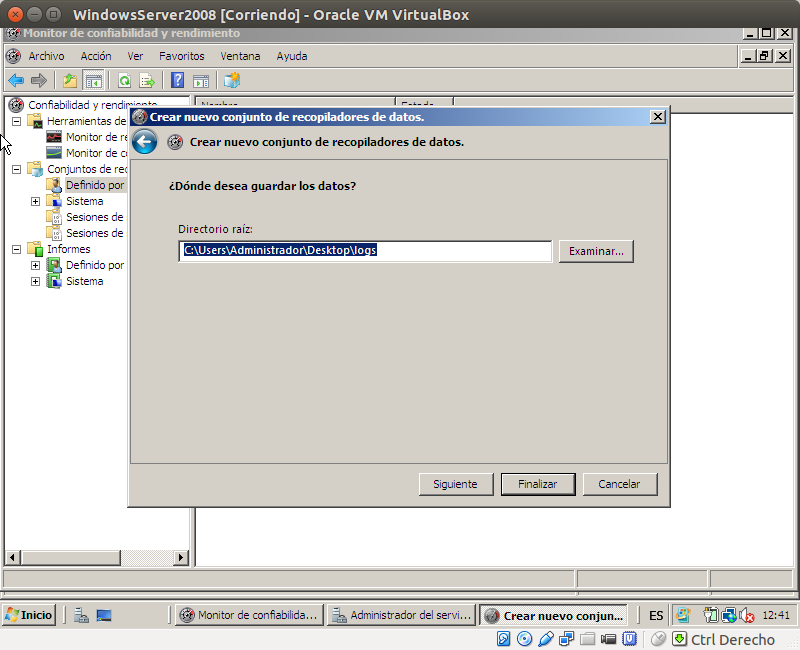
\includegraphics[width=0.6\linewidth]{EscritorioLogs}
		\caption[GuardarDatos]{Guardar los datos en el $/Escritorio/logs$ ($/Descktop/logs$).}
		\label{fig:EscritorioLogs}
		\end{figure}
		
		Ahora ya tenemos creado nuestro recopilador de datos, pero para que este comience a monitorizar, tenemos que iniciar el seguimiento:\\
		\begin{figure}[H]
		\centering
		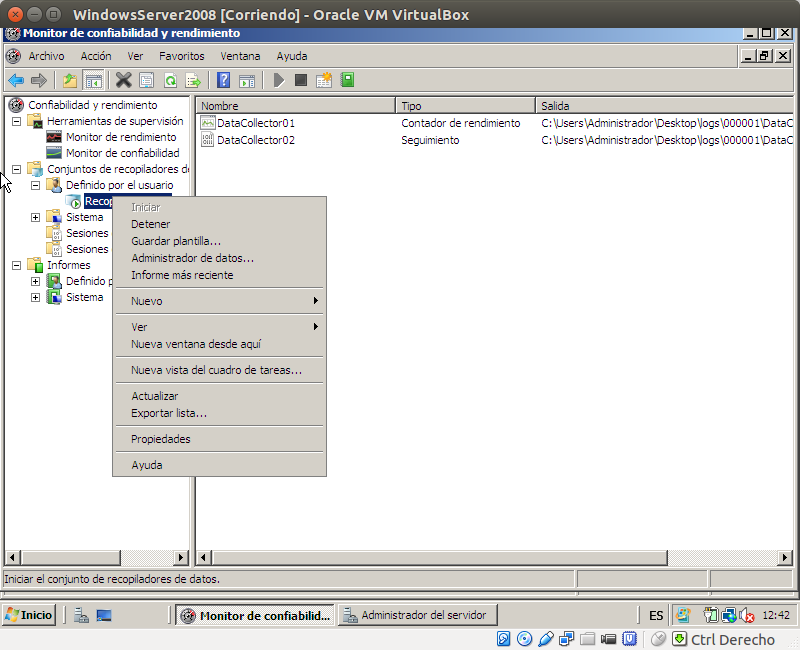
\includegraphics[width=0.6\linewidth]{seguimiento}
		\caption[Seguimiento]{Iniciar seguimiento con click derecho->Iniciar.}
		\label{fig:seguimiento}
		\end{figure}
		
		Nos vamos al directorio donde hemos guardado el monitor y lo ejecutamos:\\
		
		\begin{figure}[H]
			\centering
			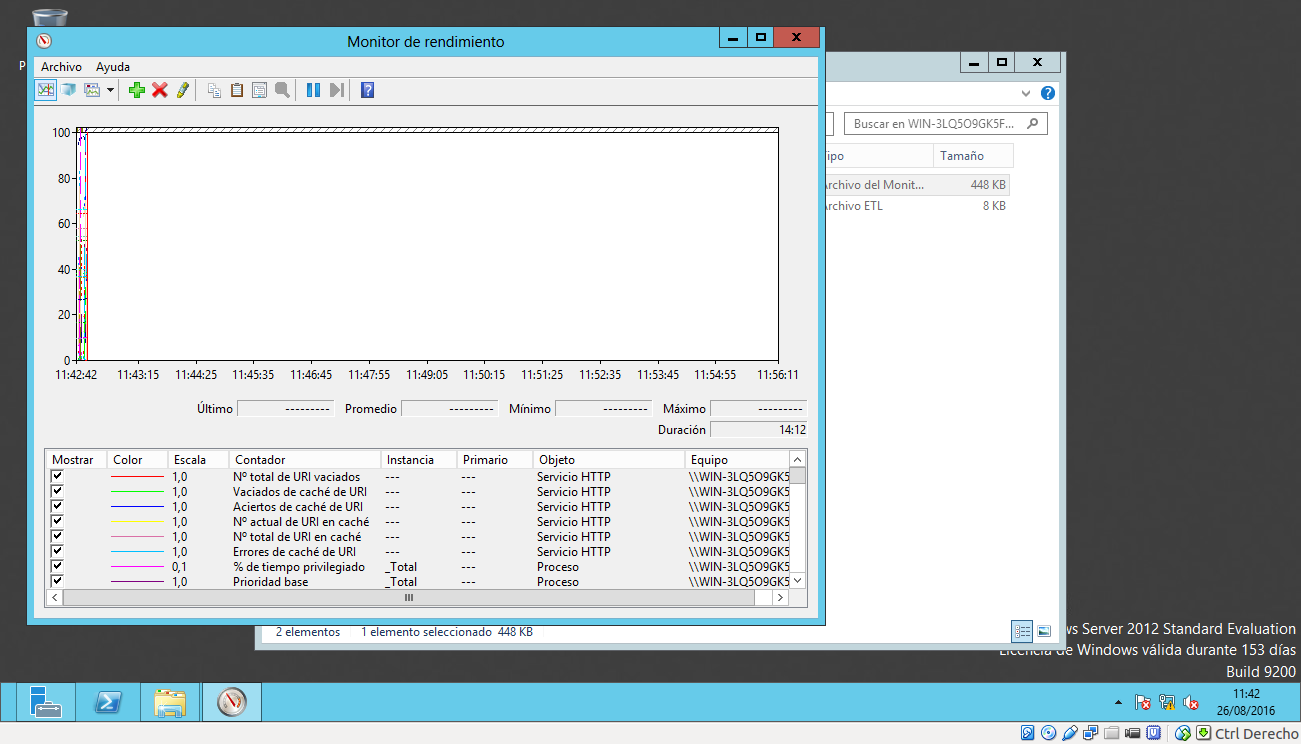
\includegraphics[width=0.7\linewidth]{MonitorEnEjecucion}
			\caption[Monitor en ejecución]{Monitor de rendimiento en ejuecución.}
			\label{fig:MonitorEnEjecucion}
		\end{figure}
		
		Como vemos, la gráfica está demasiado llena. Deseleccionando algunas de ellas:\\
		\begin{figure}[H]
			\centering
			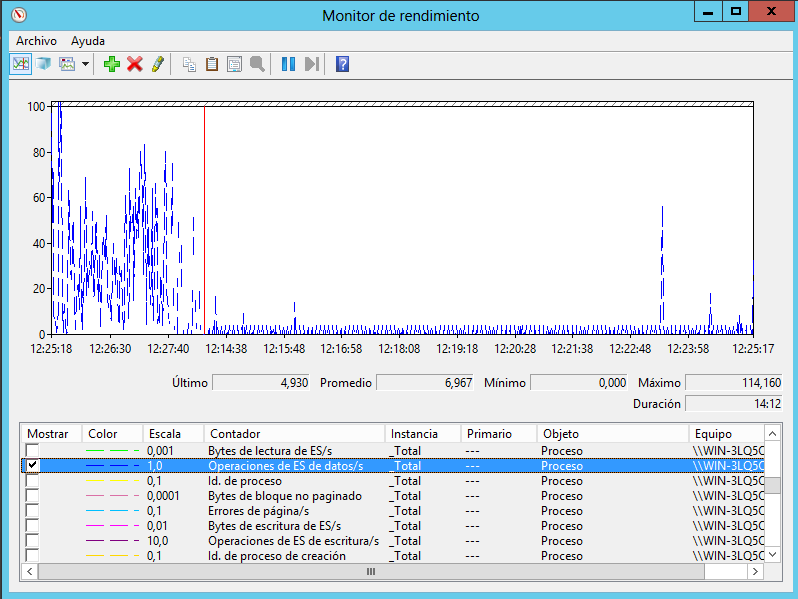
\includegraphics[width=0.7\linewidth]{WindowsOperacionesES}
			\caption[OperacionES]{Operaciones de entrada y salida en el sistema.}
			\label{fig:WindowsOperacionesES}
		\end{figure}
		
		 obtenemos la gráfica de un aspecto concreto. En la gráfica mostrada se ilustra el número de operaciones de entrada/salida por segundo del sistema. Podemos ver el número medio de operaciones, la última medición realizada y otros datos estadísticos de estas mediciones. Ej: El número de operaciones entrada/salida por segundo máximo que ha realizado el sistema es de más de 114 operaciones por segundo.
		

		
\end{itemize}

\section{Monitorización del Hardware.}

\begin{itemize}
	\item \textbf{Instale alguno de los monitores comentados arriba en su máquina y
		pruebe a ejecutarlos (tenga en cuenta que si lo hace en la máquina virtual, los
		resultados pueden no ser realistas). Alternativamente, busque otros monitores para
		hardware comerciales o de código abierto para Windows y Linux.}\\
	El primer monitor instalado en el sistema de $hddtemp$ \cite{hddtemp}, que nos muestra la temperatura de los discos duros de nuestro PC en Linux. Tras ejecutar $hddtemp$ sobre un disco duro en concreto(En nuestro caso $/dev/sda$), nos puede salir una salida como la siguiente:\\
	
	$/dev/sda:$ $ST500LM012$ $HN-M500MBB:$ $48ºC$\\
	
	en el cual nos muestra que la temperatura del mismo es 48 grados celsius. Mas información en el manual, antes citado.\\
	
	Para detectar los sensores de la placa base necesitamos instalar la librería $lm-sensors$ \cite{sensors}(la página del proyecto está caida). Esta librería es necesaria para el siguiente monitor gráfico del sistema, psensor, que se instala con el paquete del mismo nombre. Este monitor nos ofrece de forma gráfica la información sobre temperatura y porcentaje de la CPU usado. Un ejemplo de la interfaz es la siguiente:\\
	
	\begin{figure}[H]
	\centering
	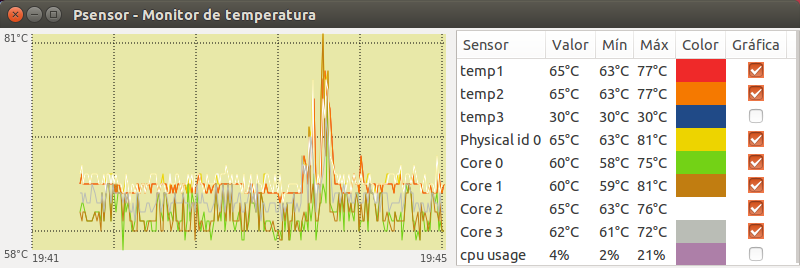
\includegraphics[width=0.7\linewidth]{psensor}
	\caption[psensor]{Gráfica que muestra psensor sobre la temperatura de algunos componentes del sistema.}
	\label{fig:psensor}
	\end{figure}
	
	Además de estos, se pueden encontrar en \cite{HWMon} otras herramientas de monitorización, como por ejemplo Hardinfo\cite{hardinfo}, que es una aplicación libre la cual muestra información acerca de los distintos componentes del sistema como el procesador, distintos dispositivos como USB's, o incluso realizar benchmarking sobre los mismos.\\
	
	
	En Windows\cite{WMonitor}, algunas de las herramientas que podemos usar para monitorizar el sistema en lugar de las ya dadas son las siguientes, entre otros:\\
	\begin{itemize}
		\item Prime95\cite{prime95}, que se encarga de cargar de trabajo todos los núcleos para comprobar su rendimiento.
		\item MemTest86\cite{memtest86}, utilizado para testear la memoria RAM.
	\end{itemize}
\end{itemize}

\section{Otros monitores de sistema.}
\subsection{Munin}
\begin{itemize}
	\item \textbf{Visite la web del proyecto y acceda a la demo que proporcionan(http://demo.munin-monitoring.org/) donde se muestra cómo monitorizan un servidor. Monitorice varios parámetros y haga capturas de pantalla de lo que está mostrando comentando qué observa.}
	
	El primer parámetro que vamos a monitorizar es el uso de la CPU. La siguiente imagen nos dice cual es el porcentaje usado por distintos consumidores al día:\\
	
	\begin{figure}[H]
	\centering
	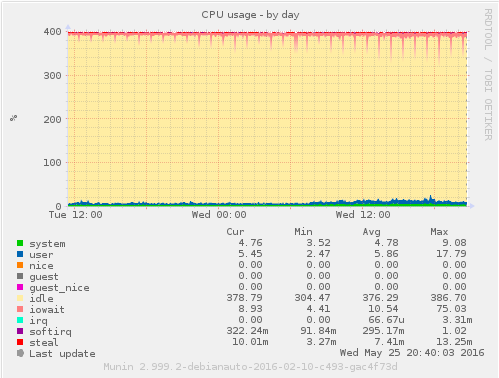
\includegraphics[width=0.7\linewidth]{monitoring_munin_cpu}
	\caption[CPUusage]{Uso de la CPU durante un día en el servidor que monitoriza Munin}
	\label{fig:monitoring_munin_cpu}
	\end{figure}
	
	En el se muestra los usos que ha tenido la CPU. Entre ellos, está el porcentaje de uso de la CPU de el usuario user, que es de alrededor del 5.48%.\\
	
	Otro parámetro a monitorizar que nos ofrece Munin es el número de procesos y el estado de los mismos:\\
	
	\begin{figure}[H]
	\centering
	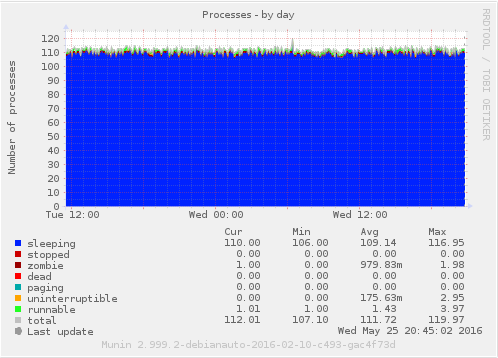
\includegraphics[width=0.7\linewidth]{monitorin_munin_procesos}
	\caption[ProcesosMunin]{Número de procesos y estado de los mismos.}
	\label{fig:monitorin_munin_procesos}
	\end{figure}
	
	En este gráfico vemos que hay alrededor de 110 procesos lanzados de los cuales la gran mayoría está $sleeping$, o esperando a estar corriendo. También vemos que apenas han quedado procesos zombies. Es importante notar que siempre hay al menos un proceso ejecutandose.\\
	
	\begin{figure}[H]
		\centering
		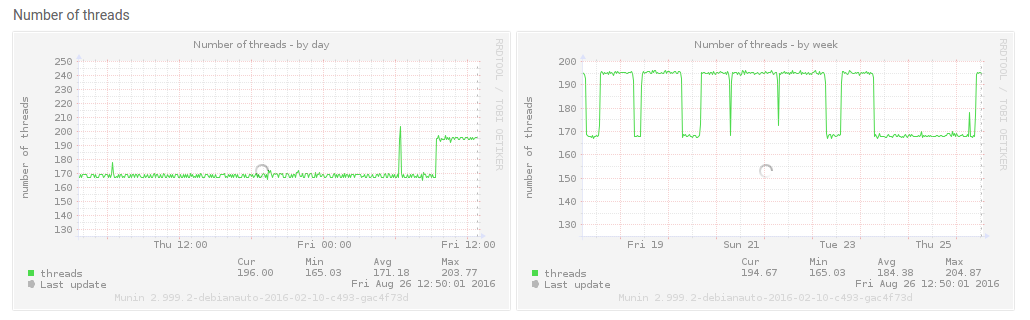
\includegraphics[width=0.7\linewidth]{MuninHebras}
		\caption[HebrasMunin]{Número de hebras que hay en cada momento en el servidor.}
		\label{fig:MuninHebras}
	\end{figure}

	Este parámetro nos indica el número de hebras en cada momento. Los dos gráficos nos muestran distintas intervalos de tiempo: por día y por semana. Hay alrededor de 171.32 hebras de media en el día de hoy en contraste con una media de 184 hebras en la semana. Esto es debido a que a lo largo de la semana ha tenido más hebras que hoy.\\
	
	Por último, en el parámetro experimental:\\
	
	\begin{figure}[H]
		\centering
		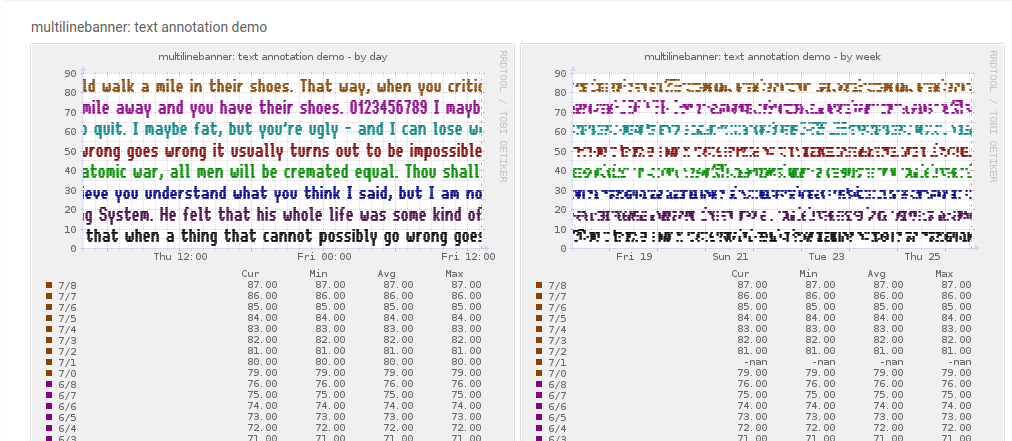
\includegraphics[width=0.7\linewidth]{MuninExperimental}
		\caption[MuninExperimental]{Parámetro Experimental de Munin.}
		\label{fig:MuninExperimental}
	\end{figure}
	
	que a priori parece que está hecho para anotar en una gráfica texto con sentido. No tengo más datos sobre este parámetro.
	
	
\end{itemize}
\subsection{Zabbix}
\begin{itemize}
	\section{ZABBIX ME FALTA}
	\item \textbf{Prueba a instalar este monitor es alguno de sus tres sistemas. Realice capturas de pantalla del proceso de instalación y comente capturas de pantalla del programa en ejecución.}\\
	
	Para instalar el monitor de zabbix he consultado los manuales de la página\cite{zabbix} para descargar este desde paquetes. Para empezar tenemos que añadir a la lista de repositorios el repositorio de este proyecto:\\
	
	$wget$ $http://repo.zabbix.com/zabbix/3.0/ubuntu/pool/main/z/zabbix-release/zabbix$-$	release\_3$.$0$-$1$+$trusty\_all.deb$ \\
	$dpkg$ -$i$ $zabbix-release_3.0$-$1+trusty_all.deb$\\
	$apt$-$get$ $update$\\
	
	Tras lo cual podremos instalar los paquetes necesarios para el servidor de zabbix:\\
	
	$apt$-$get$ $install$ $zabbix$-$server$-$mysql$ $zabbix$-$frontend$-$php$ $zabbix$-$agent$\\
	
	Para tener zabbix inicializado con una base de datos ya creada, se nos facilita un ejemplo que podemos utilizar para comprobar que está funcionando. Para ello, ejecutamos el siguiente script que nos facilita la página:\\
	
	shell> mysql -uroot -p<password>\\
	mysql> create database zabbix character set utf8 collate utf8\_bin;\\
	mysql> grant all privileges on zabbix.* to zabbix@localhost identified by '<password>';\\
	mysql> quit;\\
	
	En el manual, parecen otros archivos como schema.sql, data.sql y images.sql que no los encontramos en el directorio donde nos indican. Esto es porque Ubuntu tiene preparado un script para ello:
	
	$/usr/share/doc/zabbix$-$server$-$mysql$:\\
	$zcat$ $create.sql.gz$ | $mysql$ -$uroot$ $zabbix$\\
	
	Ahora, como cada vez que instalamos un servicio, debemos asegurarnos que está configurado como queremos, o como nos aconsejan que lo tengamos en la página web del proyecto. Para ello modificamos con nuestro editor favorito su archivo de configuración y descomentamos las siguientes líneas de opciones y añadimos lo necesario para que estas opciones queden en el archivo:\\

	$DBHost=localhost$\\
	$DBName=zabbix$\\
	$DBUser=zabbix$\\
	$DBPassword=zabbix$\\
	
	tras lo cual, como debemos hacer cuando modificamos el archivo de configuración de cualquier servicio, lo reiniciamos:\\
	
	$service$ $zabbix$-$server$ $restart$\\
	
	El último retoque que debemos hacer para terminar de configurar zabbix es descomentar la linea de zona horario en apache2 y poner nuestra zona horaria. Por supuesto, tras esto, reiniciamos apache:\\
	
	$service$ $apache2$ $restart$\\
	
	Ahora ya podremos entrar en zabbix desde cualquier navegador, en localhost/zabbix/setup.php:\\
	
	\begin{figure}[H]
	\centering
	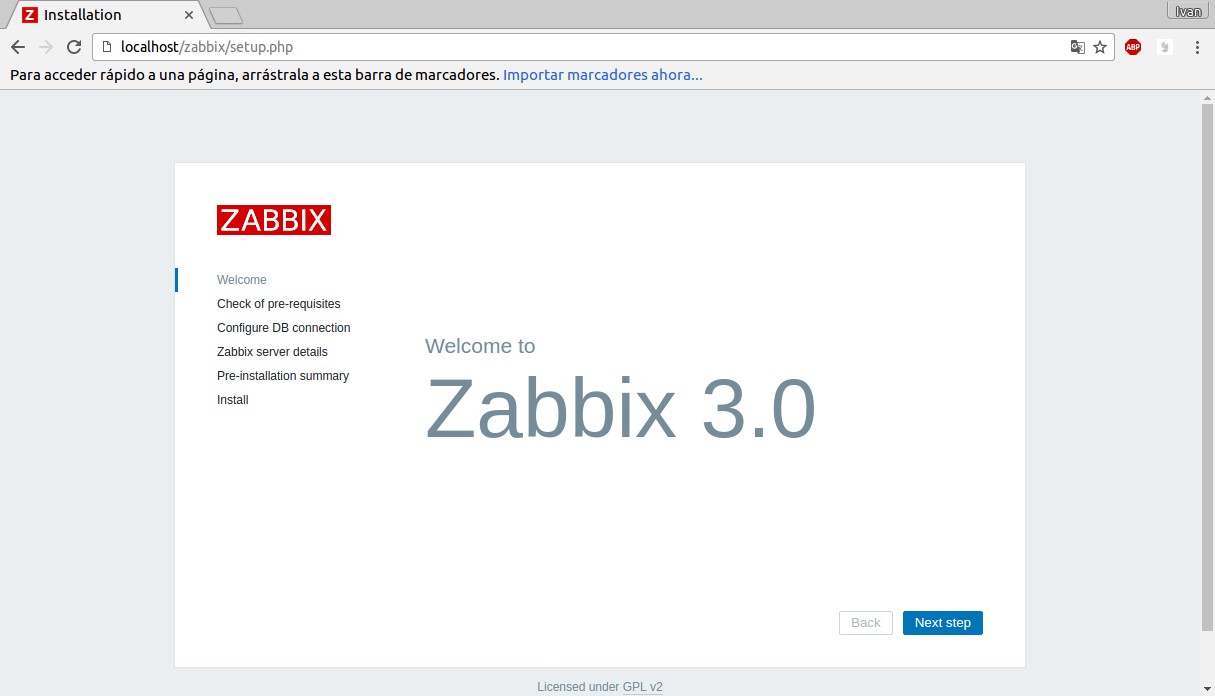
\includegraphics[width=0.7\linewidth]{zabbix1}
	\caption[Inicio de zabbix]{Ventana que aparece la primera vez que te conectas a zabbix.}
	\label{fig:zabbix1}
	\end{figure}
	
	Ahora nos mostrarán unas opciones de configuración que deberemos rellenar:\\
	
	\begin{figure}[H]
	\centering
	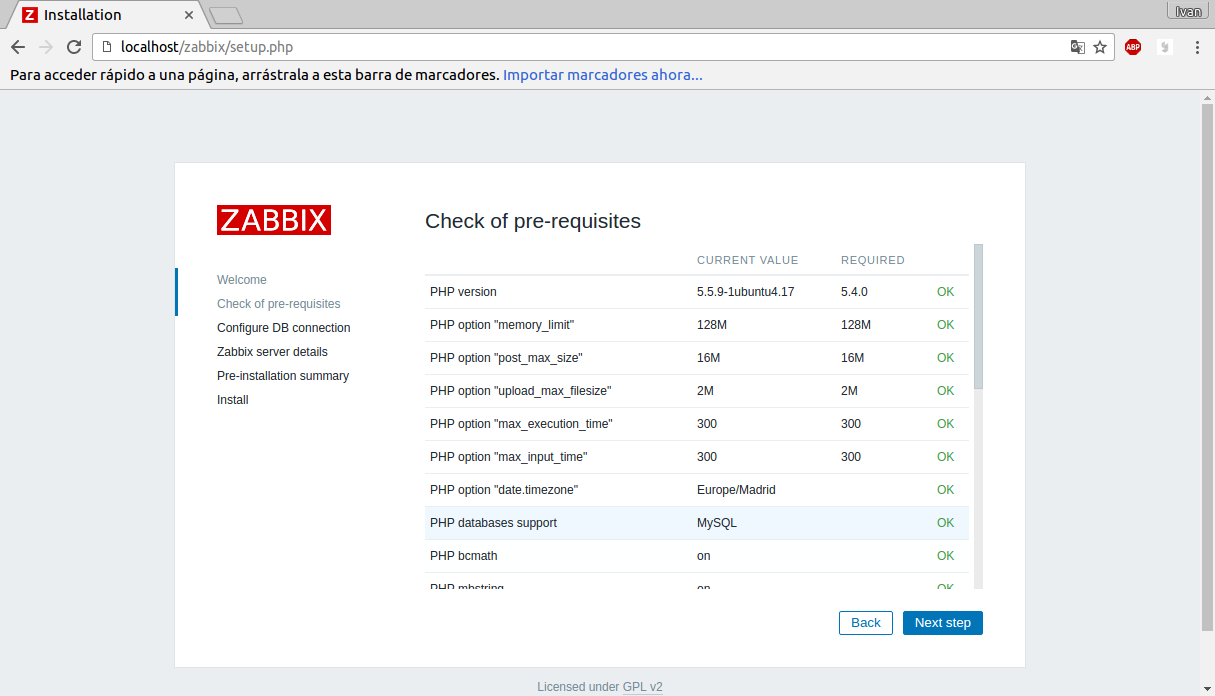
\includegraphics[width=0.7\linewidth]{zabbix2}
	\caption[zabbix2]{Opciones por defecto de zabbix.}
	\label{fig:zabbix2}
	\end{figure}
	
	\begin{figure}[H]
	\centering
	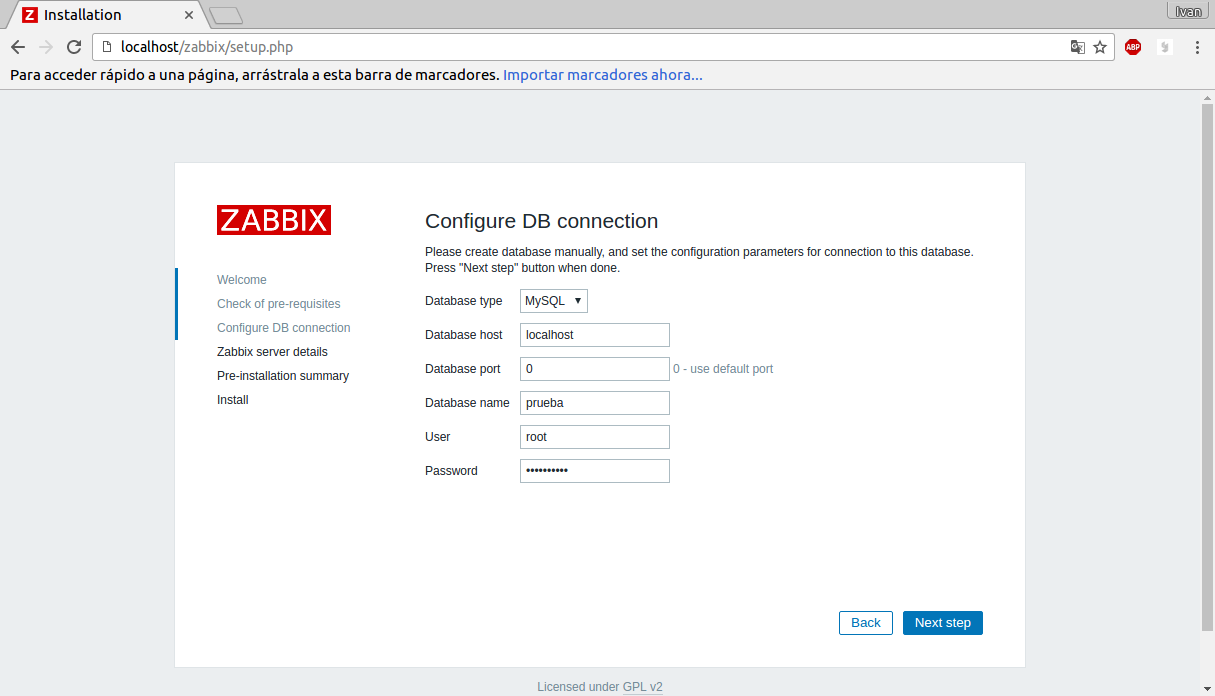
\includegraphics[width=0.7\linewidth]{zabbix3}
	\caption[zabbix3]{Usuario de mysql.}
	\label{fig:zabbix3}
	\end{figure}
	
	\begin{figure}[H]
	\centering
	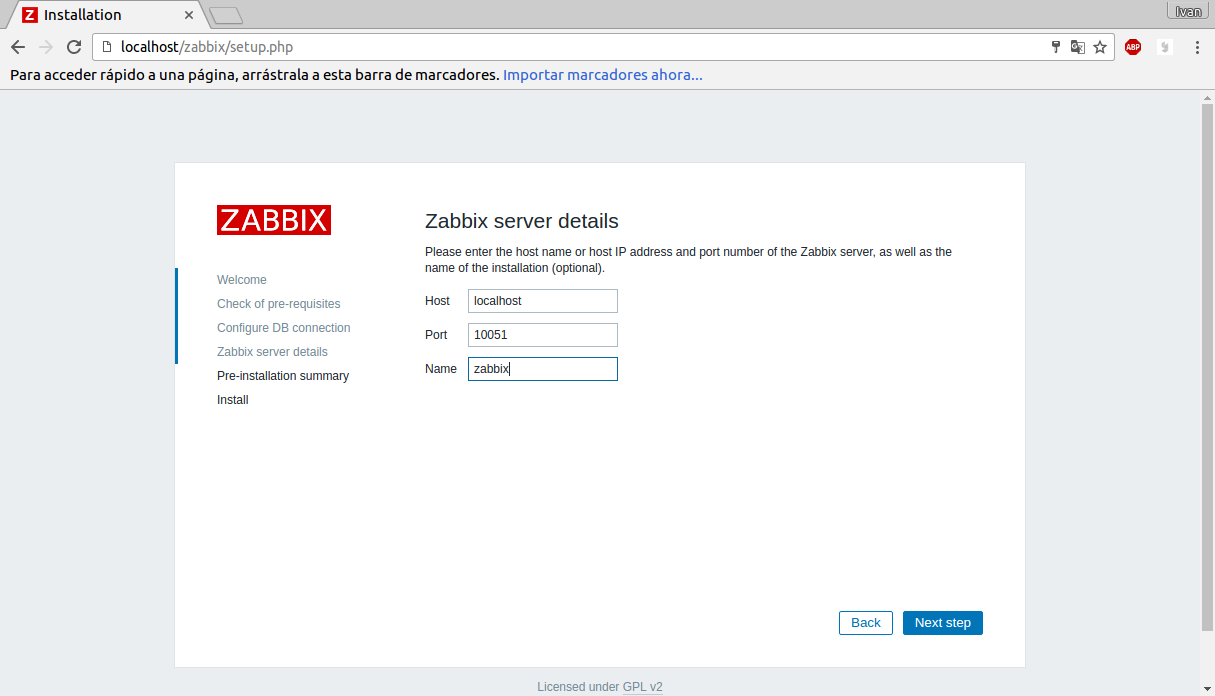
\includegraphics[width=0.7\linewidth]{zabbix4}
	\caption[zabbix4]{Usuario y contraseña usada para zabbix. Por defecto Admin/zabbix}
	\label{fig:zabbix4}
	\end{figure}
	
	\begin{figure}[H]
	\centering
	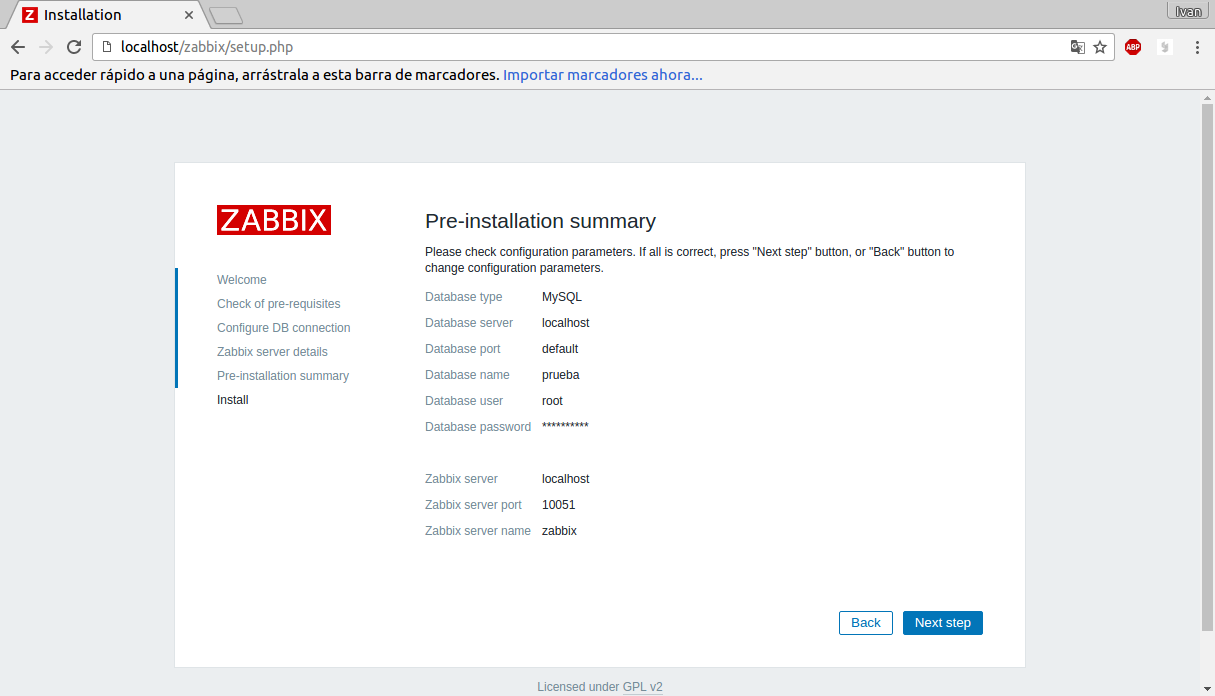
\includegraphics[width=0.7\linewidth]{zabbix5}
	\caption[zabbix5]{Sumario de la instalación.}
	\label{fig:zabbix5}
	\end{figure}
	
	\begin{figure}[H]
	\centering
	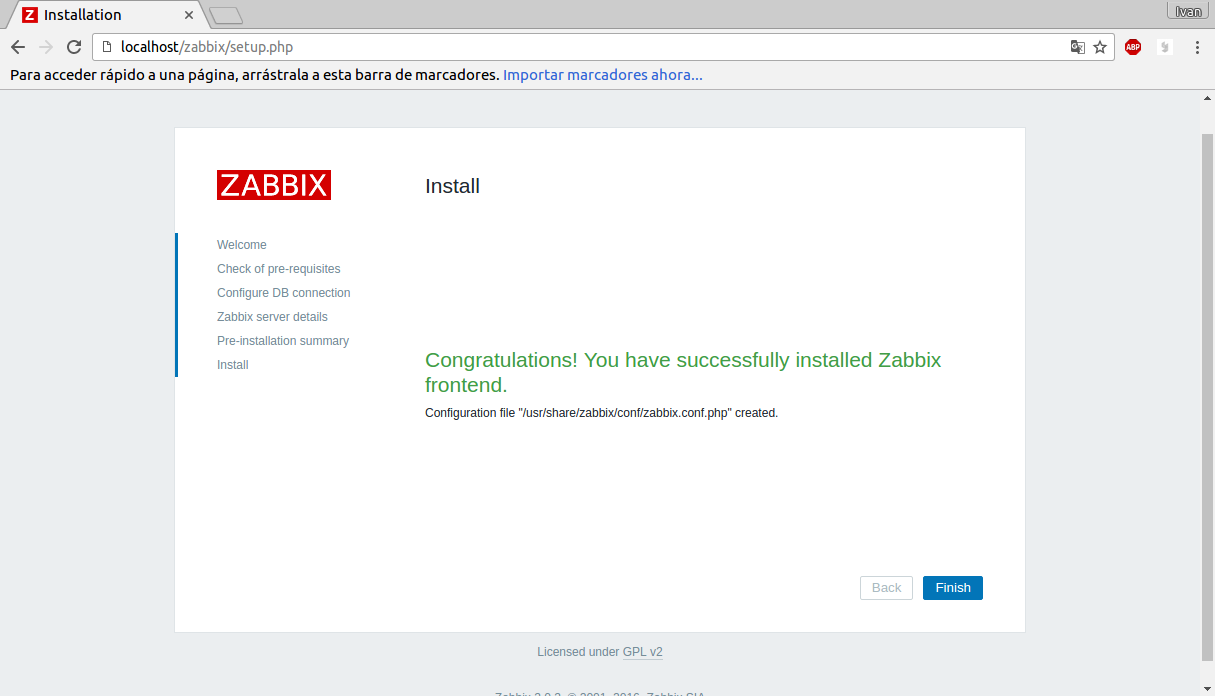
\includegraphics[width=0.7\linewidth]{zabbix6}
	\caption[zabbix6]{Configuración completada.}
	\label{fig:zabbix6}
	\end{figure}
	
	\begin{figure}[H]
	\centering
	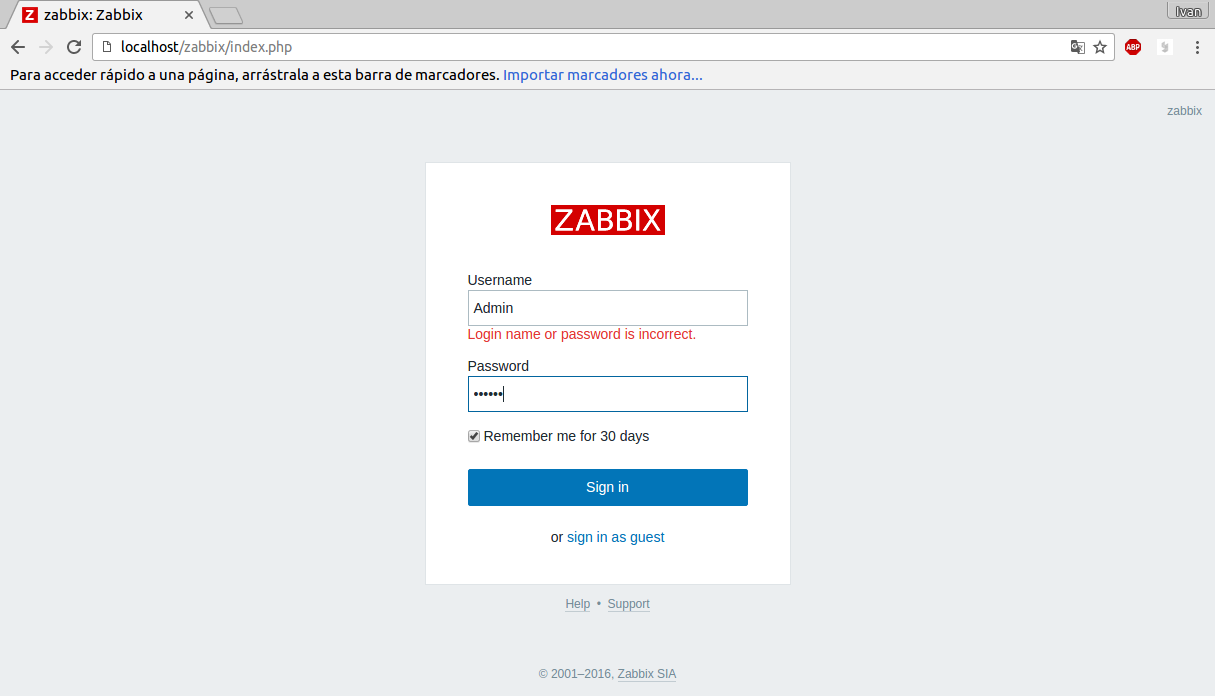
\includegraphics[width=0.7\linewidth]{zabbix7}
	\caption[zabbix7]{Entrar por primera vez en zabbix}
	\label{fig:zabbix7}
	\end{figure}
	
	Una vez nos registramos, nos aparece la siguiente interfaz:\\
	\begin{figure}[H]
	\centering
	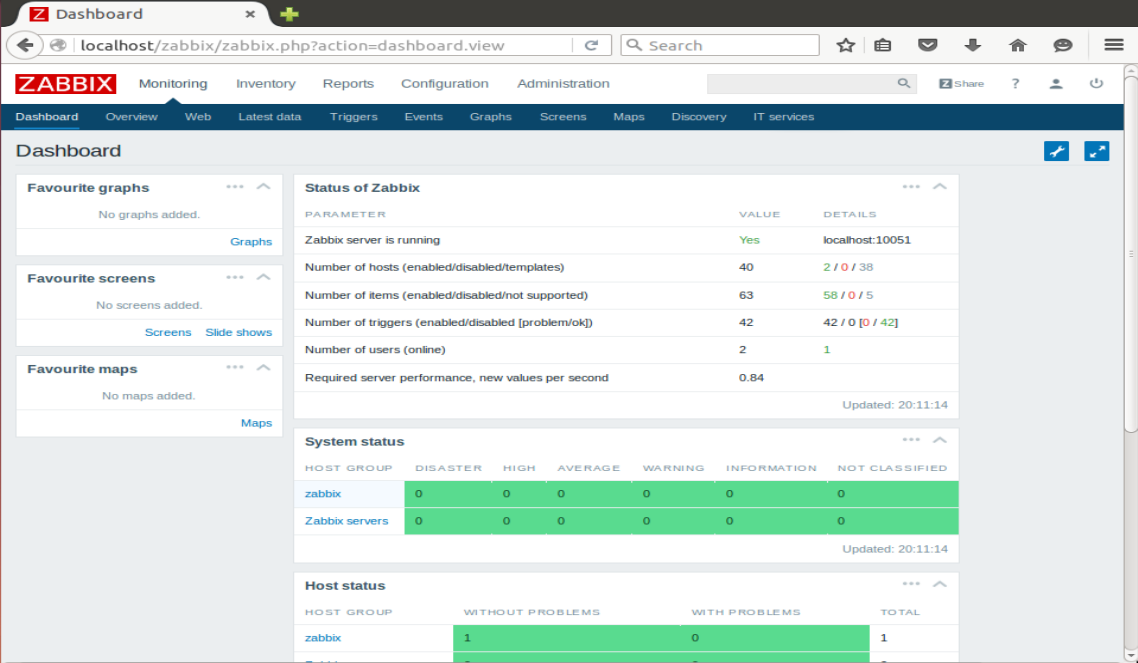
\includegraphics[width=0.7\linewidth]{zabbixPORFIN}
	\caption[Interfaz zabbix]{Interfaz general de zabbix.}
	\label{fig:zabbixPORFIN}
	\end{figure}
	
	Ahora, para monitorizar un  servicio nos vamos a la sección Graphs y seleccionamos algún servicio. Por ejemplo:\\
	\begin{figure}[H]
	\centering
	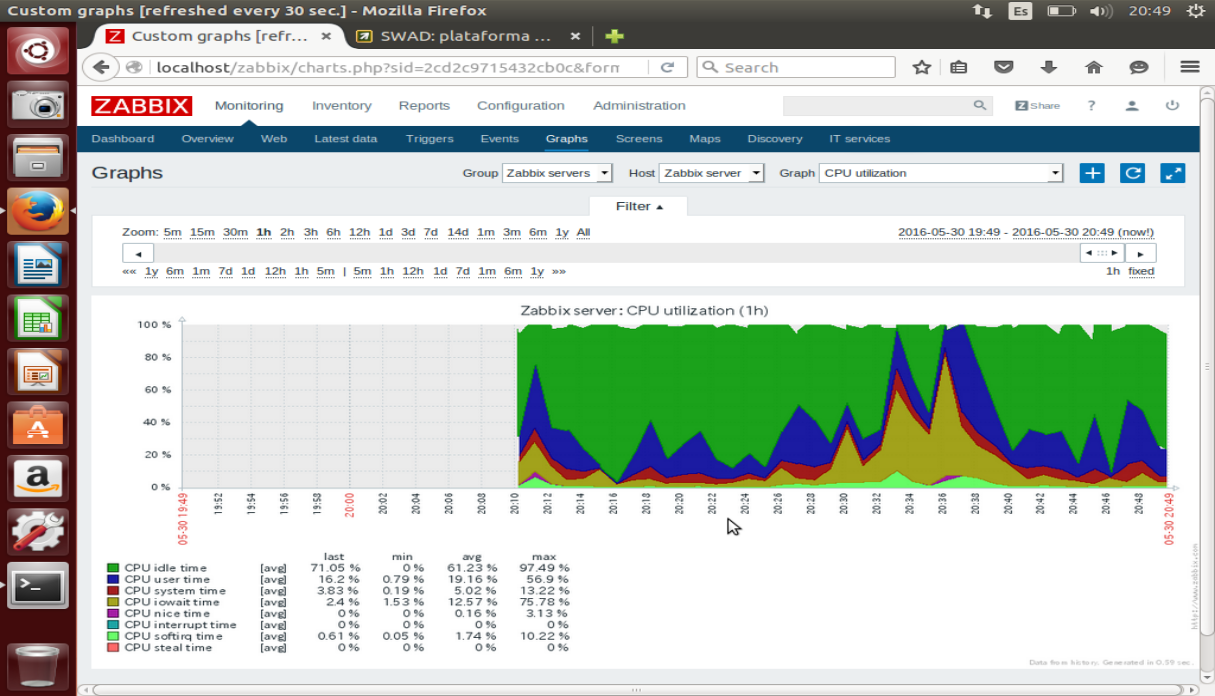
\includegraphics[width=0.7\linewidth]{CPUUsage}
	\caption[Uso de CPU]{Gráfico que muestra el porcentaje de uso de la CPU de nuestro servidor.}
	\label{fig:CPUUsage}
	\end{figure}
	Así por ejemplo vemos en verde el porcentaje de CPU no usado, en azul el usado por parte del usuario y en rojo, el porcentaje usado por el sistema en cada momento de la última hora(en realidad menos por ser inicializado hace menos de una hora).


	
	
\end{itemize}
\subsection{Cacti}

\textbf{Instale y pruebe el monitor Cacti y pruebe alguna funcionalidad del mismo.}\\


\newpage
\subsection{Monitorizando un servicio}
\begin{itemize}
	\item \textbf{Escriba un breve resumen sobre alguno de los artículos donde se muestra el uso de strace, o busque otro programa similar y coméntelo.}\\
	
	En mi caso, he visitado la página\cite{strace}, en la que se habla de algunas utilidades de strace y de un problema que el escritor solucionó gracias a este monitor de servicios. Las primeras líneas nos explican que esta herramienta no solo puede monitorizar un servicio desde el principio (lanzándolo con strace), si no que también puede lanzarse aunque el servicio ya esté ejecutándose. Esto es muy útil a la hora de monitorizar daemons que no deban ser reiniciados muy a menudo. En cuanto al problema que plantea, se resume de la siguiente manera: Se está utilizando un servicio SVN que fallaba aleatoriamente y nadie podía acceder al mismo. Reiniciar el servidor arreglaba el problema, pero no permanentemente, volvía a fallar. Al escritor se le ocurrió buscar en los archivos log, pero no había ninguno. Además, a la hora de observar cómo se iniciaban los procesos, todo parecía correcto, pero por alguna razón, el sistema se colgaba. Entonces recurrió, puesto que no podía modificar el código con opciones de debugueo, a utilizar un script que lanzara svnserver pero cazando la información que nos pueda dar strace. De esta forma, los clientes podrían seguir utilizando el servicio. Este cambio hizo visible el problema fácilmente en cuanto varios usuarios utilizaron el servicio. El problema era que a la hora de dar $filehandle$ para lectura, se daba el filehandle número 5, pero este fallaba. \\
	
	Por lo visto, este problema ocurre cuando el sistema no tiene la suficiente entropía para generar un stream aleatorio, por lo que reiniciar el sistema podría solucionar parcialmente el problema(podría "reiniciar" la entropía). El por qué de esta falta de entropía no se aclara ya que, según el autor, no era necesario. Utilizando, en vez de el generador de streams aleatorios $/dev/random$, otro generador que no fallase con la falta de entropía, $/dev/urandom$ , solucionó fácilmente el problema. En principio esto es un fallo de seguridad, pero en el trabajo que estaban realizando y según el criterio del autor, este fallo era irrelevante.\\
	
	La entrada del blog termina diciendo que este problema hubiese sido imposible de resolver sin un debugger o strace, siendo este último bastante más sencillo de utilizar.
	
\end{itemize}

\section{Profiling}
	\subsection{Python}
	\begin{itemize}
		\item \textbf{Escriba un script en python y analice su comportamiento usando el profiler presentado.}\\
		Utilizando cProfile\cite{python} como profiler para analizar el comportamiento de el siguiente script:\\
		\begin{figure}[H]
		\centering
		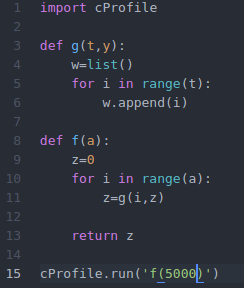
\includegraphics[width=0.4\linewidth]{pythonProgram}
		\caption[Script en python]{Script de python sobre el que vamos a realizar el profiling.}
		\label{fig:pythonProgram}
		\end{figure}
		
		nos da la siguiente salida:\\
		
		\begin{figure}[H]
		\centering
		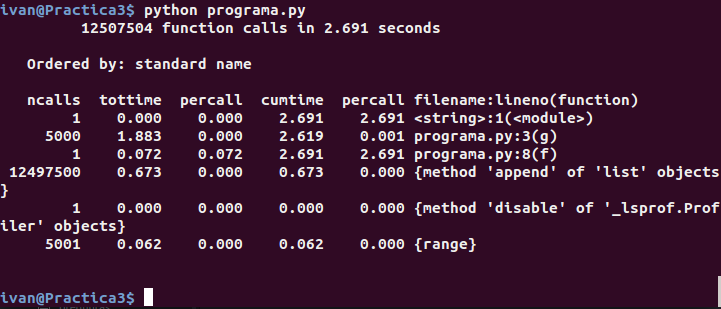
\includegraphics[width=0.8\linewidth]{python_profiling}
		\caption[profiling python]{Salida del script anterior.}
		\label{fig:python_profiling}
		\end{figure}
		
		en la cual vemos varias llamadas a cada una de las funciones que hemos creado junto con el tiempo que pasa el programa en total en cada función o en particular en cada llamada a cada función.\\
		
		\begin{itemize}
			\item Vemos que hay una función que se llama 5000 veces. Esta es la función g definida anteriormente. Esto es porque se ha llamado desde la función f 5000 veces a g. Por esta razón, vemos que el tiempo que el programa ha estado en esta función es de 1.883 segundos, pero tarda alrededor de 0.001 segundos por llamada.\\
			
			\item La función f pasa dentro de la misma(no en subllamadas) alrededor de 0.072 segundos. Sin embargo, el tiempo total que el programa está en esta función y en subllamadas del mismo es 2.691 segundos.\\
			
			\item La función append de listas es llamada 124975 veces. Esto es porque en cada subllamada a la función g se llama muchas veces a la función append.
		\end{itemize}
		
		Estas son algunas de las anotaciones que se pueden hacer del profiling que hemos realizado del programa en python.

	\end{itemize}

\subsection{Bases de datos}

\begin{itemize}
	\item \textbf{Acceda a la consola mysql (o a través de phpMyAdmin) y muestre el
		resultado de mostrar el ”profile” de una consulta (la creación de la BD y la consulta la
		puede hacer libremente)}\\
	
	Tras observar cómo usar el comando SHOW PROFILE y SHOW PROFILES en mysql\cite{mysqlProfile,mysqlProfiles}, para los cuales es necesario cambiar a 1(true) la variable profiling para que estas puedan trabajar, y haber hecho la creación de dos bases de datos, la inserción de unos cuantos datos y unas cuantas consultas pertinentes, el resultado de ejecutar ambos comandos son los siguientes:\\
	\begin{figure}[H]
	\centering
	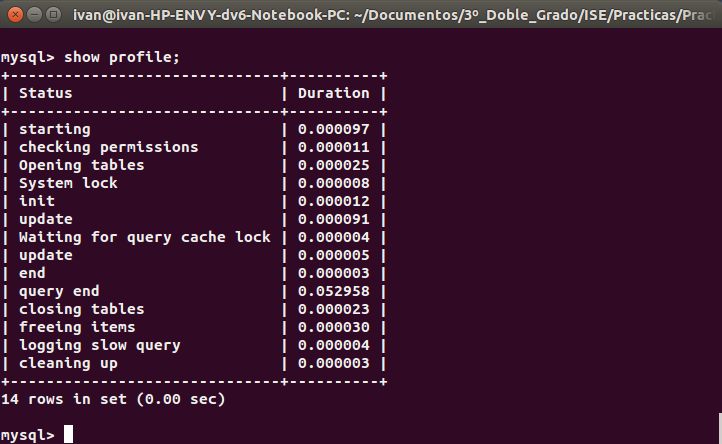
\includegraphics[width=0.7\linewidth]{mysqlProfile}
	\caption[mysqlProfile]{Salida en mysql tras ejecutar SHOW PROFILE.}
	\label{fig:mysqlProfile}
	\end{figure}
	
	Con este comando podemos ver los tiempos de carga, inicio, comprobación de permisos, etc... que realiza la base de datos. Ahora veamos cuanto ha tardado la base de datos en concreto en realizar las consultas y la creación de tablas:\\
	\begin{figure}[H]
	\centering
	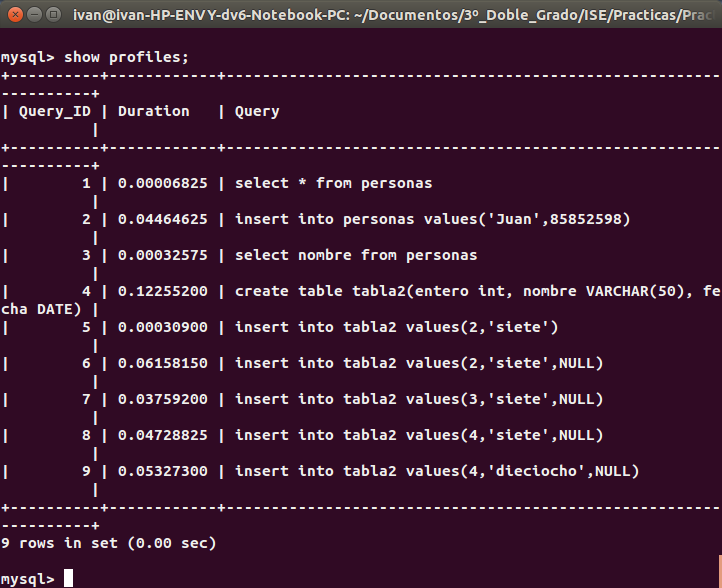
\includegraphics[width=0.7\linewidth]{mysqlProfiles}
	\caption[mysqlProfiles]{Salida en mysql tras ejecutar SHOW PROFILES.}
	\label{fig:mysqlProfiles}
	\end{figure}
	Aquí podemos ver los tiempos que ha tardado en cada una de las operaciones que le hemos ordenado que haga. En la misma, podemos ver que la creación de la tabla ha tardado alrededor de una décima de segundo y que en las inserciones, ha tardado alrededor de media décima. También vemos que al realizar mal una consulta, descartarla ha sido rápido. \\
	
	Un dato curioso es que a la hora de mostrar la primera tabla completa  ha tardado menos que en mostrar solo parte de la misma. Esto se debe a que a la hora de filtrar parte de la tabla se gasta más tiempo que en mostrar todo directamente.

\end{itemize}
\newpage
\begin{thebibliography}{xx}
	\bibitem{crontab} http://linux.die.net/man/1/crontab
	\bibitem{hddtemp} http://linux.die.net/man/8/hddtemp
	\bibitem{sensors} http://www.tecmint.com/psensor-monitors-hardware-temperature-in-linux/
	\bibitem{HWMon} http://www.educadictos.com/herramientas-de-monitorizacion-de-hardware-para-ubuntu-12-04/
	\bibitem{hardinfo} http://www.guia-ubuntu.com/index.php/HardInfo
	\bibitem{WMonitor} http://hardzone.es/programas-para-testear-monitorizar-y-comprobar-el-rendimiento-de-tu-pc/
	\bibitem{prime95} http://www.mersenne.org/
	\bibitem{memtest86} http://www.memtest86.com/
	\bibitem{nagios} https://www.nagios.org/
	\bibitem{strace} https://debian-administration.org/article/352/Using\_strace\_to\_debug\_application\_errors
	\bibitem{mysqlProfile} http://dev.mysql.com/doc/refman/5.7/en/show-profile.html
	\bibitem{mysqlProfiles} http://dev.mysql.com/doc/refman/5.7/en/show-profiles.html
	\bibitem{zabbix} https://www.zabbix.com/documentation/3.0/manual/installation/install\_from\_packages
	\bibitem{python} https://docs.python.org/2/library/profile.html
	
\end{thebibliography}
\end{document}